% The five selection rules on one example clip with n = 20 valid frames and k = 3.
% SME and positional frames follow Section 4.4 (f_1, f_11, f_20 and f_4, f_11, f_17; study guide 9.3).
% The random, k-Changepoint, and k-BOCPD frames are only an example: they differ from clip to clip.
% k-BOCPD can score only frames with 7 valid frames on each side (frames 8-14 of 20), and peaks must be
% at least 7 apart, so on a clip this short it keeps a single frame (Section 4.4).
\documentclass[12pt,border=10pt]{standalone}
% Shared style for the slide figures: sans-serif text (Helvetica, close to the Arial of the charts),
% the same colors as charts.py, and the manuscript's table tools.
\usepackage[T1]{fontenc}
\usepackage[scaled]{helvet}
\renewcommand{\familydefault}{\sfdefault}
\usepackage{amsmath,amssymb}
\usepackage{sansmath}
\usepackage{xcolor}
\usepackage{booktabs,array}
\newcolumntype{L}[1]{>{\raggedright\arraybackslash}p{#1}}
\usepackage{tikz}
\usetikzlibrary{arrows.meta,positioning,calc}

\definecolor{ink}{HTML}{0B0B0B}
\definecolor{inktwo}{HTML}{52514E}
\definecolor{muted}{HTML}{898781}
\definecolor{gridc}{HTML}{E1E0D9}
\definecolor{basec}{HTML}{C3C2B7}
% one color per selection rule, in the fixed categorical order of the charts
\definecolor{cp}{HTML}{2A78D6}     % k-Changepoint (content)
\definecolor{sme}{HTML}{EB6834}    % SME (position)
\definecolor{posc}{HTML}{1BAF7A}    % positional (position)
\definecolor{rnd}{HTML}{EDA100}    % random (chance)
\definecolor{bocpd}{HTML}{E87BA4}  % k-BOCPD (content), categorical slot 5
\definecolor{temporal}{HTML}{6250D6}  % temporal information added to the mean (frame combinations figure)

\newcommand{\chip}[1]{\tikz[baseline=0.1ex]\fill[#1, rounded corners=1pt] (0,0) rectangle (0.32cm,0.32cm);}
\AtBeginDocument{\sansmath\color{ink}}
\hyphenpenalty=10000 \exhyphenpenalty=10000   % no hyphenated words on slides

\newcommand{\framerow}[5]{% #1 y, #2 label, #3 color, #4 selected frames, #5 note
   \node[anchor=east, align=right] at (0.2, #1) {#2};
   \foreach \i in {1,...,20} \draw[basec, line width=0.7pt, fill=white] (\i-0.4, #1-0.32) rectangle (\i+0.4, #1+0.32);
   \foreach \i in {#4} \draw[#3!70!black, line width=0.9pt, fill=#3] (\i-0.4, #1-0.32) rectangle (\i+0.4, #1+0.32);
   \node[anchor=west, font=\small, text=inktwo, align=left] at (20.75, #1) {#5};
}
\begin{document}
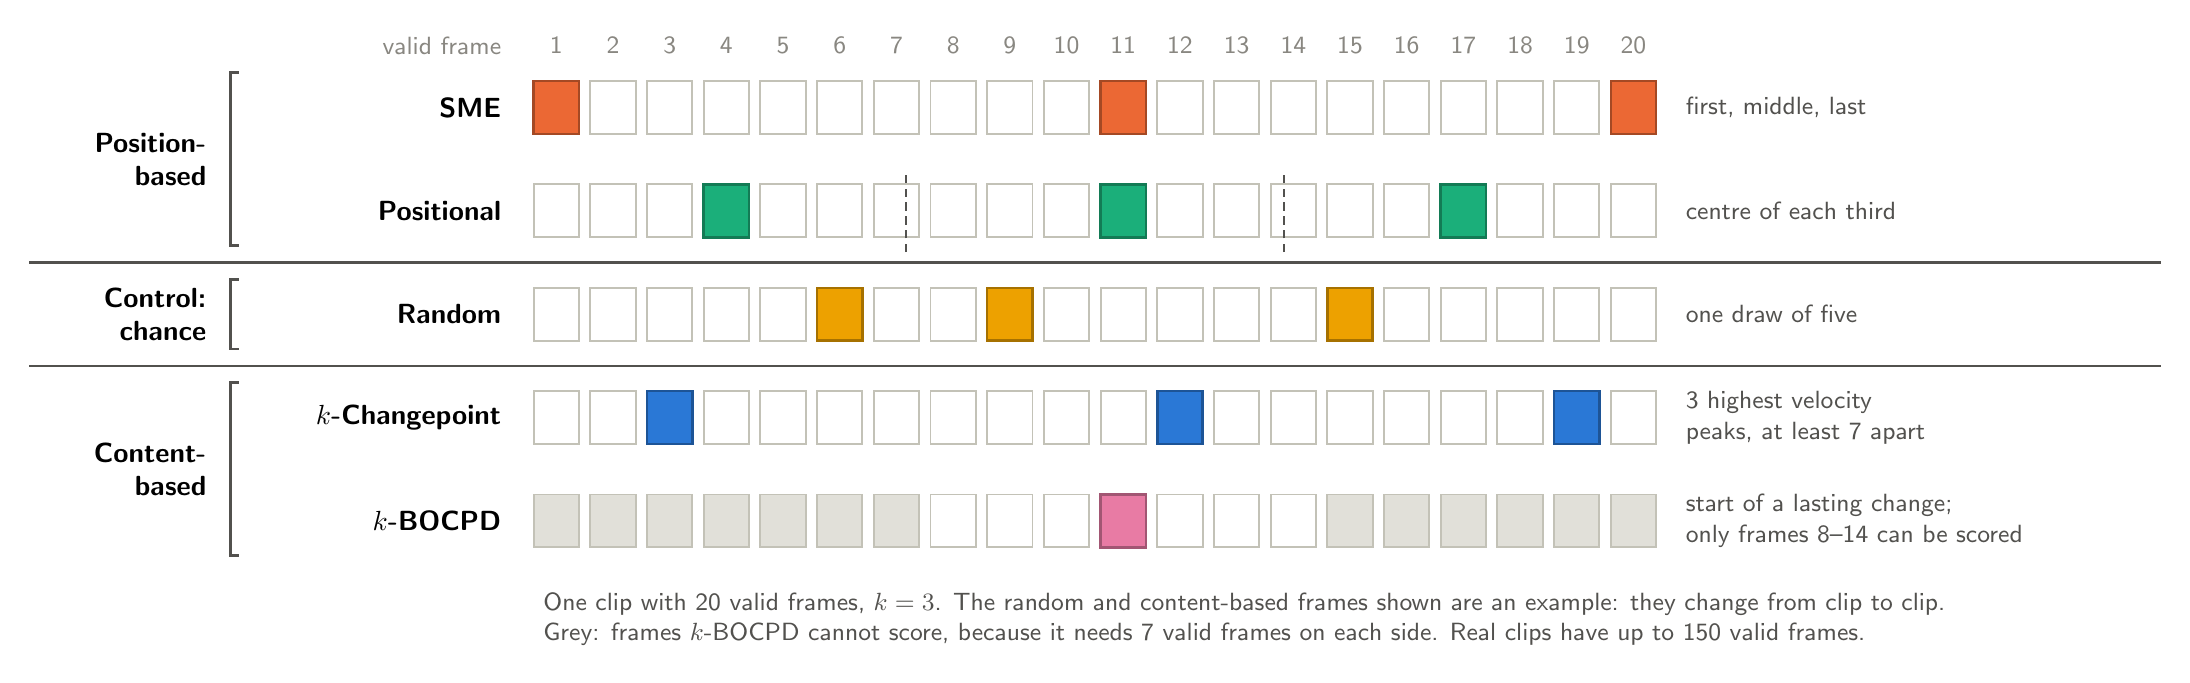
\begin{tikzpicture}[x=0.72cm, y=1.05cm]
   \foreach \i in {1,...,20} \node[font=\small, text=muted] at (\i, 0.75) {\i};
   \node[anchor=east, font=\small, text=muted] at (0.2, 0.75) {valid frame};
   \framerow{0}{\textbf{SME}}{sme}{1,11,20}{first, middle, last}
   \framerow{-1.25}{\textbf{Positional}}{posc}{4,11,17}{centre of each third}
   \framerow{-2.5}{\textbf{Random}}{rnd}{6,9,15}{one draw of five}
   \framerow{-3.75}{\textbf{$k$-Changepoint}}{cp}{3,12,19}{3 highest velocity\\peaks, at least 7 apart}
   \framerow{-5}{\textbf{$k$-BOCPD}}{bocpd}{11}{start of a lasting change;\\only frames 8--14 can be scored}
   % groups (Doc Jay, 20 Nov: a clear line between the position-based and content-based rules)
   \foreach \y in {-1.875, -3.125} \draw[inktwo, line width=1pt] (-8.3, \y) -- (29.3, \y);
   \foreach \top/\bot/\lab in {0.42/-1.67/{Position-\\based}, -2.08/-2.92/{Control:\\chance}, -3.33/-5.42/{Content-\\based}} {
      \draw[inktwo, line width=1pt] (-4.6, \top) -- (-4.75, \top) -- (-4.75, \bot) -- (-4.6, \bot);
      \node[anchor=east, align=right, font=\bfseries] at (-5.0, {(\top+\bot)/2}) {\lab};
   }
   % frames k-BOCPD cannot score on a 20-frame clip (fewer than 7 valid frames on one side)
   \foreach \i in {1,...,7,15,16,...,20} \fill[gridc] (\i-0.4, -5-0.32) rectangle (\i+0.4, -5+0.32);
   \foreach \i in {1,...,7,15,16,...,20} \draw[basec, line width=0.7pt] (\i-0.4, -5-0.32) rectangle (\i+0.4, -5+0.32);
   % the three equal segments of positional selection
   \foreach \b in {7.1667, 13.8333} \draw[inktwo, line width=0.9pt, dash pattern=on 3pt off 2pt] (\b, -1.25-0.5) -- (\b, -1.25+0.5);
   \node[anchor=north west, font=\small, text=inktwo, align=left] at (0.6, -5.75)
      {One clip with 20 valid frames, $k = 3$. The random and content-based frames shown are an example: they change from clip to clip.\\
       Grey: frames $k$-BOCPD cannot score, because it needs 7 valid frames on each side. Real clips have up to 150 valid frames.};
\end{tikzpicture}
\end{document}
